\begin{tikzpicture}
\begin{axis}[
  height=5cm, width=10cm,
  xmin=-3.5, xmax=3.5,
  ymin=0, ymax=0.50,
  ytick={0},
  axis x line=bottom, axis y line=center,
  xlabel=$x$, ylabel=$f(x)$,
  every axis x label/.style={at={(current axis.right of origin)},anchor=north west},
  every axis y label/.style={at={(current axis.above origin)},anchor=north west}
]

% Draw normal curve
\addplot[blue,thick,smooth,domain=-3.5:3.5] {
  (1/(sqrt(2*pi)))*exp(-(x^2)/2) 
};

% Draw vertical line:
\only<2->{
  \draw [red,thick] (axis cs:-1.5,0) -- (axis cs:-1.5,0.1295176);
}

% Draw area
\only<3->{
  \addplot[fill=blue,opacity=0.4,smooth,domain=-3.225:-1.51] { (1/(sqrt(2*pi)))*exp(-(x^2)/2) } \closedcycle;
}
\end{axis}
\end{tikzpicture}
